\chapter{Feasibility of Learning}\label{Sec:Feasibility of Learning}

No practical amount of data can distinguish between two distributions, thus instances of GBS can not be proven to come from GESIS. However, machine learning allows to infer the conditional probability of \textit{'GBS participant is representative'} given the survey data within a probabilistic framework. A well-defined learning problem involves a number of design choices, including selecting the target function to be learned, a representation for this target function, and an algorithm to learn from the source of training experience \cite{tom}. This paper defines key terminology of the theoretical aspects of survey analysis and machine learning. The MRS algorithm is then formulated as positive-unlabeled learning problem in addition to traditional machine learning.

\section{Sampling Bias}

Variables considered in the GBS study must accurately reflect the populations characteristics. That is, every element of the population has a known non-zero chance of being selected. This includes people whether or not they choose to take part in the survey. Results can then be used to make estimates for not only the sample itself but also the target population. A sampling method is called biased if it systematically favors some people over others, e.g. by oversampling people with strong opinions and undersampling people who do not care much about the topic of the survey \cite{west}.

Sampling bias is often referred to as selection bias or sample selection bias. I will stick to the more descriptive term sampling bias. It underlines the fact that the bias arises in how the data was sampled. Also, the use of the term becomes less ambiguous, because there exists another notion of selection bias in the context of model selection. This type of bias is usually referred to as bad generalization, where the performance of the selected hypothesis is overly optimistic \cite{yaser}.

\section{The Problem of Overfitting}

Overfitting stands out as one of the biggest challenges for machine learning. It is not exclusive to machine learning but rather a fundamental problem across science and is at the very heart of the dangers of statistical inference. Hypothesis \(h\) in \(H\) overfits training data if there exists an alternative hypothesis \(\bar{h}\) in \(H\) such that \(errorTrain(h) < errorTrain(\bar{h})\) and \(errorD(h) > errorD(\bar{h})\), where \(errorTrain(h):=\) error of hypothesis \(h\) over training data and \(errorD(h):=\) error over entire distribution \(D\) of data. A hypothesis overfits the training examples if some other hypothesis that fits the training examples less well actually performs better over the entire distribution of instances \cite{yaser}.

When overfitting occurs, the learned hypothesis is very good at calculating the answers for the given data, but much less so for new instances it encounters. It often occurs when the algorithm has too many options to play with in approximating the target function. The freedom to tune parameters and add complexity until it exactly matches the training data, rather than looking for large, systematic patterns leads to high variance \cite{yaser}. The error rate on the training data, the resubstitution error, as turned out to be overly optimistic, is not a good indicator of performance on future data. A fair way to properly estimate error rates is to use cross-validation as a powerful general technique. The expected prediction error at any given data point \(x_0\), the generalization error, can be decomposed as follows \cite{ian}: 
\begin{align*}
Err(x_o) &= \EX[(Y - \bar{f}(x_0))^2 \mid X = x_0] \\
& =  \sigma^2_\epsilon + [\EX\bar{f}(x_0) - f(x_0)]^2 + \EX[\bar{f}(x_0) - \EX\bar{f}(x_0)]^2\\
& =  \sigma^2_\epsilon + Bias^2(\bar{f}(x_0)) + Var(\bar{f}(x_0)) \\
& = Irreducible Error + Bias^2 + Variance
\end{align*}

The bias and variance terms make up the error of \(\bar{f}(x_0)\) in estimating \(f(x_0)\). The bias component is the squared difference between the true mean \(f(x_0)\) and the expected value of the estimate \([\EX\bar{f}(x_0) - f(x_0)]^2\), where the expectation averages the randomness in the training data. The variance term refers to the amount by which the estimate of the target function would change if it was estimated using a different training data set. Ideally the estimate for the underlying pattern should not vary too much between training sets. More generally, as the model complexity is increased, the variance tends to increase and the squared bias tends to decrease. The opposite behavior occurs as the model complexity is decreased. The first term in this expression is the irreducible error, a combination of stochastic and deterministic noise. More precisely, stochastic noise are fluctuations or measurement errors that can not be modelled. Re-measuring \(y_n\) changes this component. Deterministic noise is the part of the target function that can not be represented. Changing \(H\) changes this component. With a single dataset \(D\) and fixed \(H\) it is impossible to distinguish \cite{yaser}.  

\section{Learning from Positive and Unlabeled Data}

\vspace{0.4cm}
\begin{algorithm}[H]
\caption{PU training procedure}\label{alg:alg}
\vspace{0.2cm}
\KwIn{\(P\): set of positive instances (GESIS)}
\myinput{\(U\): set of unlabeled instances (GBS)}
\myinput{\(n_{models}\): number of base models in ensemble}
\myinput{\(n_P\): size of bootstrap sample of \(P\)}
\myinput{\(n_U\): size of bootstrap sample of \(U\)}
\KwResult{Scoring function \(f:U \rightarrow \) $\mathbb{R}$}
Initialize: 
\(f(x) \leftarrow 0\) and 
\(c(x) \leftarrow 0\)\\
\For{t = 1 to \(n_{models}\)}{
\hfill \\
  Draw a bootstrap sample \(P_t\) of size \(n_P\). \\
  Draw a bootstrap sample \(U_t\) of size \(n_U\). \\
  Train classifier \(f_t\) to discriminate \(P_t\) against \(U_t\). \\
  For any \(x \in U \backslash U_t\), update: \\
\(f(x) \leftarrow f(x) + f_t(x),\) \\ 
\(c(x) \leftarrow c(x) + 1\) \\
\vspace{0.2cm}}
Return: \(s(x) = f(x)/c(x)\)
\vspace{0.3cm}
\end{algorithm}
\vspace{0.4cm}

Training a binary classifier in a semi-supervised way from only positive and unlabeled sample points is called PU learning. A positive set \(P\) and mixed set \(U\), which is assumed to contain positive and negative samples, are available for training. A variety of techniques exist to adapt supervised classifiers to the PU learning setting. PU learning is used for tasks such as matrix completion and multi-view learning. It can also be used in data mining to classify data streams, time series and to detect events, like co-occurences, in graphs \cite{elkan, claesen}. 

In semi-supervised learning, the most straightforward approach to deal with positive and unlabeled data, is to assume that all the unlabeled data are negative and simply apply traditional learning techniques. It has been shown that in many practical cases the posterior distributions in traditional and non-traditional setting provide the same optimal ranking of instances on a given test sample \cite{jain, claesen}.

The first approach handles unlabeled data as negatives and derives a solution that is purely discriminative, i.e. neither GBS nor GESIS distributions are modeled explicitly. Discriminative learners will look for a decision boundary that separates participants according to the survey they have taken. Survey participants on a hold-out set are then classified as either GBS or GESIS, depending on which side of the decision boundary they fall. Predictions are made accordingly to create a ranking. The instance in GESIS with the lowest predicted probability marks the threshold for excluding every GBS instance that is ranked below.

The most extensively studied and widely used performance evaluation in binary classification involves estimating the Receiver Operating Characteristic (ROC) curve. AUROC, the area under the ROC curve, has a meaningful probabilistic interpretation that is used to the ability of the classifier to separate classes and rank instances. The ROC curve visualized the trade-offs between the classifier's performance on positive versus negative instances over a range of decision thresholds \cite{roc}. Evaluation approaches using ROC curves are insensitive to the variation of raw prediction scores unless they affect the ranking.

\vspace{1cm}
\begin{figure}[ht]
	\begin{center}
		\captionsetup{width= 380pt}
		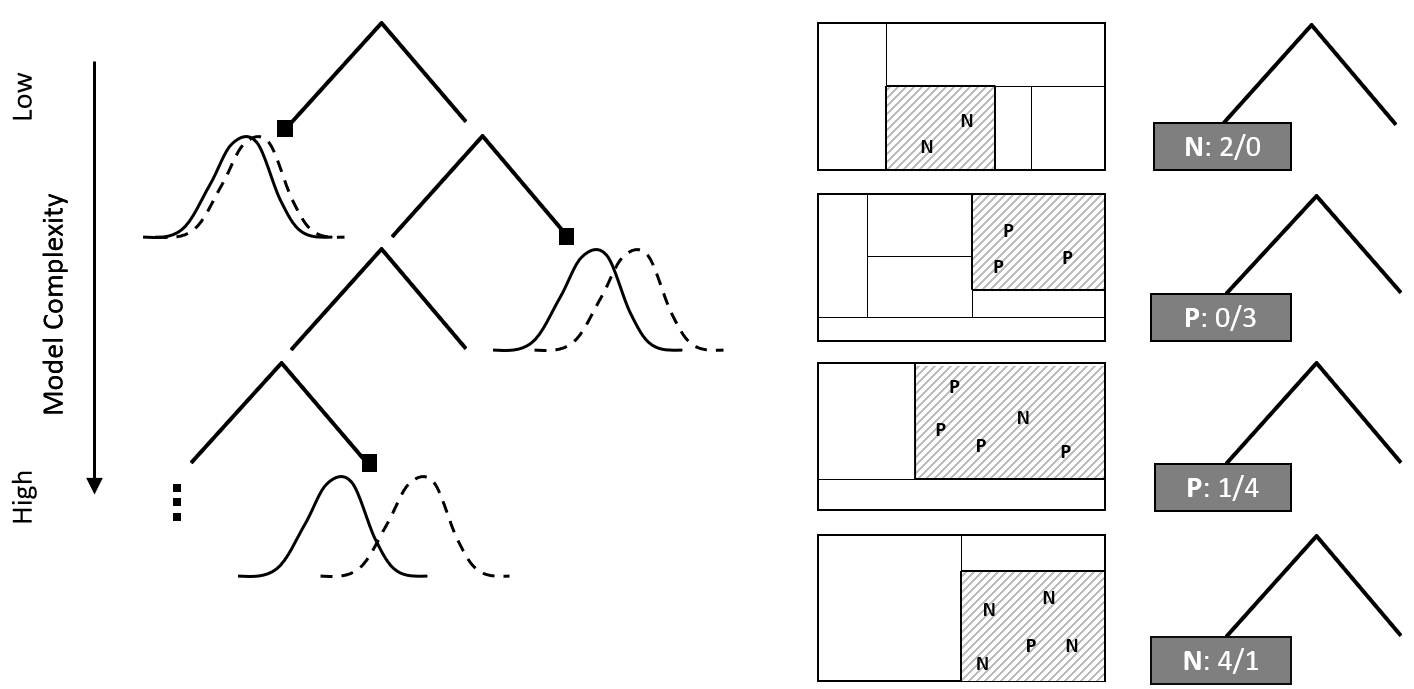
\includegraphics[scale=0.32,angle=0]{fig/tree}
		\label{project}
		\caption{Tree-based algorithm as discriminative learner. Increasing model complexity results in a better separation of GBS and GESIS and an improvement of the AUROC on the training data. Predicted probabilities are based on the proportions of positives and negatives in subspaces. Test set instances of GBS in leaf nodes are removed if correctly classified. The terms over-represented and under-represented can be translated to four distinct leaf node possibilities. If we excluded all misclassified instances, then we are also changing GESIS distribution, of which we know it is representative. Subsampling means adapting GBS distributions only.}
	\end{center}
\end{figure}

\newpage
The subsequent method PU training has been summarised in Algorithm 1. Base models are trained on resamples from both GESIS and GBS, yielding different levels of fraction of positives in the resamples. The variation of this fraction between base model training sets induces variability between base models without increasing bias. Breiman \cite{leo} introduced bagging as a technique to construct strong ensembles by combining a set of base learners. To grow a suitably diverse ensemble of base classifiers, each time a random subsample \(U_t\) of \(U\) is selected, a classifier is trained to discriminate \(P_t\) from \(U_t\), and used to assign a predictive score to any element of \(U\) that has not been used for training. A final score is obtained by aggregating the predictions of the classifiers trained on subsamples that did not contain the instance itself. Instances are then excluded following the same logic as in the previous method \cite{claesen2, jain2}.

The assigned scores to the elements of GBS reflect our confidence that these elements are representative. However, one may argue that assigning a score to an unlabeled example that has been used as negative training example is problematic. In particular, if a model overfits, a false negative will hardly be given a high training score when used as a negative. Because some of the unlabeled data in the training set are in fact positive, the described procedure results in biased AUROC estimates. In contrast to pu learning itself, estimating the true performance of a non-traditional classifier has not been thoroughly studied. Assessing the performance of binary classifiers becomes a non-trivial task in the absence of known negatives. Estimating the fraction of positives enables us to calculate an upper and a lower bound for the AUROC using the ROC curve in the positive-unlabeled setting \cite{claesen2, jain, jain2}.

Let \(f\) be the true distribution over the input space \(X\) from which unlabeled data is drawn. With distributions \(f_1\) and \(f_0\) of the positive and negative examples, respectively, it follows that \[f(x) = \alpha f_1(x) + (1-\alpha)f_0(x),\] with positive class prior \(\alpha \in [0,1], x \in X\).

Consider the binary classification problem from input \(x \in X\) to output \(y \in Y\) (representative: '\(1\)', not representative: '\(0\)'). The learning objective is to discriminate between \(X_p\) drawn according to \(f_1\) and \(X_u\) drawn according to \(f\)  and recover its performance estimate in the traditional setting, i.e. evaluating the decision boundary between positive and negative data \cite{jain}.

Recall \(\gamma\), false positive rate \(\eta\) and precision \(\rho\) are defined as: \(\gamma = P[\hat{Y} = 1| Y = 1]\), \(\eta = P[\hat{Y} = 1| Y = 0]\) and \(\rho = P[Y = 1| \hat{Y} = 1]\), where \(\hat{Y}\) is an estimate of the true class label \(Y\). TPR \(\gamma\) can be estimated directly, because \(X_p\) was sampled from \(f_1\), while this does not hold true for \(\eta\) given the absence of samples from \(f_0\). 
\begin{gather*}
\gamma = \e{f_1[h(x)]} = \frac{1}{|X_p|} \sum\nolimits_{x \in X_p} h(x) \\
\hat{\eta}^{pu} = \e{f[h(x)]} = \frac{1}{|X|} \sum\nolimits_{x \in X} h(x)
\end{gather*}

The area under ROC curves \(AUROC^{pu}\) so far could only be estimated for the positive versus unlabeled classification by plotting \(\gamma\) and \(\hat{\eta}^{pu}\). To calculate \(AUC\) from \(AUC^{pu}\), \cite{jain} express \(\eta\) in terms of \(\hat{\eta}^{pu}\) and \(alpha\) and provide a full derivation from the probabilistic definition of the AUC with
\[\eta = \frac{\hat{\eta}^{pu} - \alpha \gamma}{1 - \alpha}\] so that
\[AUC = \frac{AUC^{pu} - \frac{\alpha}{2}}{1 - \alpha}\] proving
\[AUC > AUC^{pu} \iff AUC^{pu} > \frac{1}{2}\]